% Copyright (c) 2026 Islam Ibrahim. All rights reserved.

\documentclass[tikz,border=8pt]{standalone}
\usepackage[T1]{fontenc}\usepackage{lmodern}\usepackage{amsmath}\usepackage{tikz}
\usetikzlibrary{arrows.meta,decorations.pathreplacing}
\begin{document}
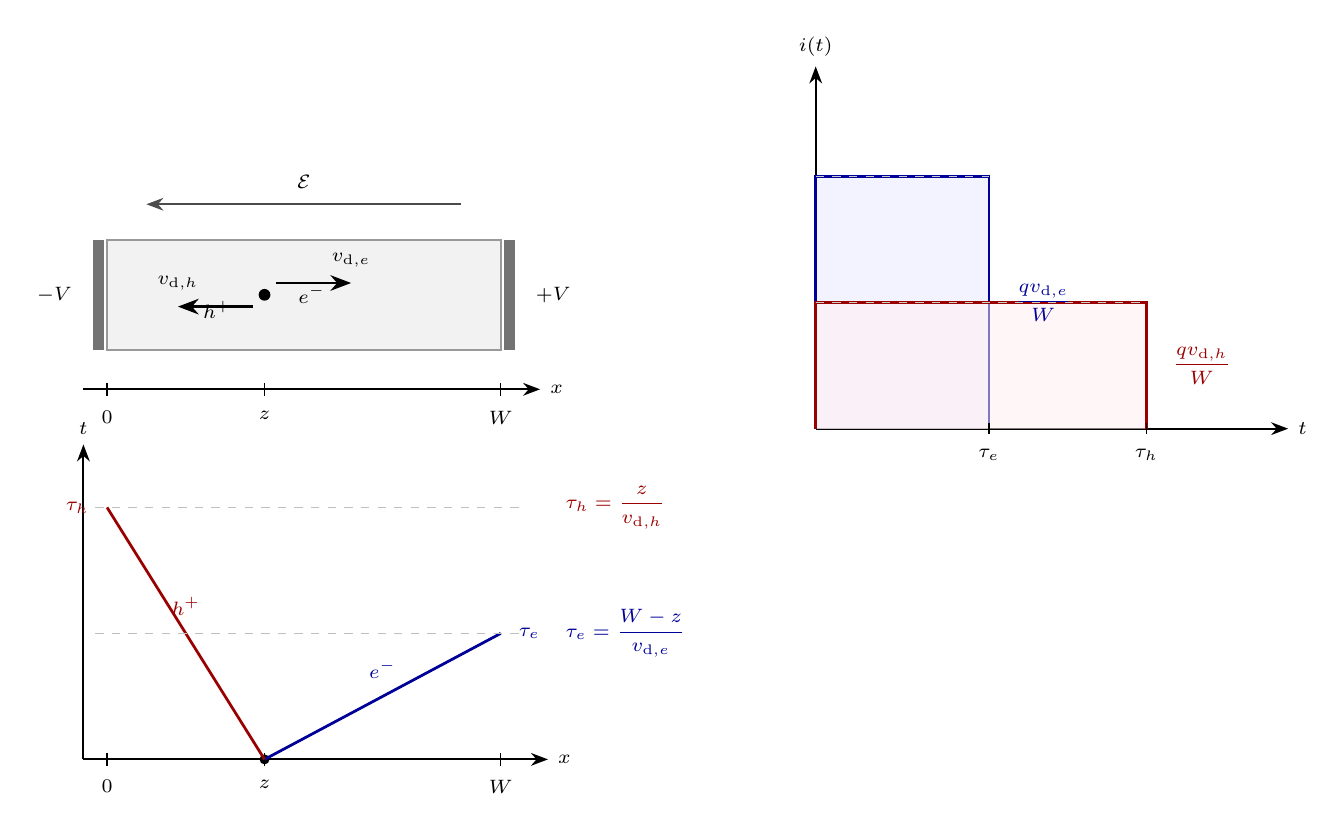
\begin{tikzpicture}[font=\small\rmfamily,>=Stealth,
  lbl/.style={font=\scriptsize\rmfamily},
  ax/.style={line width=0.7pt,->},
  seg/.style={line width=1.0pt},
  ec/.style={circle,fill=black,inner sep=1.5pt},
]

% ============================================================
% (a) Device schematic
% ============================================================
\begin{scope}
  \def\W{5.0}
  \def\devH{1.4}
  \def\zpos{2.0}

  % Depletion / intrinsic region
  \fill[gray!10,draw=black!40,line width=0.6pt]
    (0,0) rectangle (\W,\devH);

  % Electrode contacts
  \fill[black!55] (-0.18,0) rectangle (-0.04,\devH);
  \fill[black!55] (\W+0.04,0) rectangle (\W+0.18,\devH);

  % Polarity labels
  \node[lbl,left=4pt] at (-0.18,\devH/2) {$-V$};
  \node[lbl,right=4pt] at (\W+0.18,\devH/2) {$+V$};

  % Electric field arrow
  \draw[line width=0.7pt,->,black!70]
    (\W-0.5,\devH+0.45) -- (0.5,\devH+0.45);
  \node[lbl,above=2pt] at (\W/2,\devH+0.45)
    {$\mathcal{E}$};

  % Electron at z — drifts right
  \node[ec] at (\zpos,\devH/2) {};
  \draw[seg,->] (\zpos+0.15,\devH/2+0.15) -- (\zpos+1.1,\devH/2+0.15)
    node[above=2pt,lbl]{$v_{\mathrm{d},e}$};
  \node[lbl,above=2pt] at (\zpos+0.6,\devH/2-0.3) {$e^-$};

  % Hole at z — drifts left
  \draw[seg,->] (\zpos-0.15,\devH/2-0.15) -- (\zpos-1.1,\devH/2-0.15)
    node[above=2pt,lbl]{$v_{\mathrm{d},h}$};
  \node[lbl,above=2pt] at (\zpos-0.6,\devH/2-0.5) {$h^+$};

  % Position axis
  \draw[ax] (-0.3,-0.5) -- (\W+0.5,-0.5)
    node[right,lbl]{$x$};
  \draw[line width=0.5pt] (0,-0.42)--(0,-0.58);
  \draw[line width=0.5pt] (\zpos,-0.42)--(\zpos,-0.58);
  \draw[line width=0.5pt] (\W,-0.42)--(\W,-0.58);
  \node[lbl,below=2pt] at (0,-0.58) {$0$};
  \node[lbl,below=2pt] at (\zpos,-0.58) {$z$};
  \node[lbl,below=2pt] at (\W,-0.58) {$W$};
\end{scope}

% ============================================================
% (b) Space-time trajectories
% ============================================================
\begin{scope}[yshift=-52mm]
  \def\W{5.0}
  \def\zpos{2.0}
  \def\taueVis{1.6}
  \def\tauhVis{3.2}

  % Axes
  \draw[ax] (-0.3,0) -- (\W+0.6,0)
    node[right,lbl]{$x$};
  \draw[ax] (-0.3,0) -- (-0.3,4.0)
    node[above,lbl]{$t$};

  % Position ticks
  \draw[line width=0.5pt] (0,-0.08)--(0,0.08);
  \draw[line width=0.5pt] (\zpos,-0.08)--(\zpos,0.08);
  \draw[line width=0.5pt] (\W,-0.08)--(\W,0.08);
  \node[lbl,below=4pt] at (0,0) {$0$};
  \node[lbl,below=4pt] at (\zpos,0) {$z$};
  \node[lbl,below=4pt] at (\W,0) {$W$};

  % Pair generation point
  \fill[black] (\zpos,0) circle(1.8pt);

  % Electron trajectory
  \draw[seg,blue!60!black] (\zpos,0) -- (\W,\taueVis);
  \node[lbl,blue!60!black,right=3pt] at (\W,\taueVis)
    {$\tau_e$};

  % Hole trajectory
  \draw[seg,red!60!black] (\zpos,0) -- (0,\tauhVis);
  \node[lbl,red!60!black,left=3pt] at (0,\tauhVis)
    {$\tau_h$};

  % Dashed time markers
  \draw[gray!50,dashed,line width=0.5pt]
    (-0.15,\taueVis) -- (\W+0.3,\taueVis);
  \draw[gray!50,dashed,line width=0.5pt]
    (-0.15,\tauhVis) -- (\W+0.3,\tauhVis);

  % Carrier labels
  \node[lbl,blue!60!black,above=3pt]
    at ({(\zpos+\W)/2},\taueVis/2) {$e^-$};
  \node[lbl,red!60!black,above=3pt]
    at (\zpos/2,\tauhVis/2) {$h^+$};

  % Transit-time definitions — more clearance from plot
  \node[lbl,blue!60!black,anchor=west] at (\W+0.7,\taueVis)
    {$\tau_e = \dfrac{W - z}{v_{\mathrm{d},e}}$};
  \node[lbl,red!60!black,anchor=west] at (\W+0.7,\tauhVis)
    {$\tau_h = \dfrac{z}{v_{\mathrm{d},h}}$};
\end{scope}

% ============================================================
% (c) Induced current impulse response
% ============================================================
\begin{scope}[xshift=90mm,yshift=-10mm]
  \def\taueC{2.2}
  \def\tauhC{4.2}
  \def\hE{3.2}
  \def\hH{1.6}

  % Axes
  \draw[ax] (0,0) -- (0,4.6)
    node[above,lbl]{$i(t)$};
  \draw[ax] (0,0) -- (6.0,0)
    node[right,lbl]{$t$};

  % Electron current pulse
  \fill[blue!8,opacity=0.6] (0,0) rectangle (\taueC,\hE);
  \draw[seg,blue!60!black]
    (0,0) -- (0,\hE) -- (\taueC,\hE) -- (\taueC,0);

  % Hole current pulse
  \fill[red!6,opacity=0.5] (0,0) rectangle (\tauhC,\hH);
  \draw[seg,red!60!black]
    (0,0) -- (0,\hH) -- (\tauhC,\hH) -- (\tauhC,0);

  % Amplitude labels — further right
  \node[lbl,blue!60!black,right=6pt] at (\taueC,\hE/2)
    {$\dfrac{qv_{\mathrm{d},e}}{W}$};
  \node[lbl,red!60!black,right=6pt] at (\tauhC,\hH/2)
    {$\dfrac{qv_{\mathrm{d},h}}{W}$};

  % Time-axis ticks
  \draw[line width=0.5pt] (\taueC,0.07)--(\taueC,-0.07);
  \draw[line width=0.5pt] (\tauhC,0.07)--(\tauhC,-0.07);
  \node[lbl,below=4pt] at (\taueC,0) {$\tau_e$};
  \node[lbl,below=4pt] at (\tauhC,0) {$\tau_h$};

  % Dashed reference lines
  \draw[gray!40,dashed,line width=0.4pt]
    (0,\hE) -- (\taueC,\hE);
  \draw[gray!40,dashed,line width=0.4pt]
    (0,\hH) -- (\tauhC,\hH);
\end{scope}

\end{tikzpicture}
\end{document}
